\documentclass[../ProjectDocumentation.tex]{subfiles}
%Gummi|065|=)
\title{\textbf{Application Design}}
\author{Kyle Lemmon}
\date{}
\graphicspath{{../}}
\begin{document}

\maketitle

\begin{figure}[h]
\centering
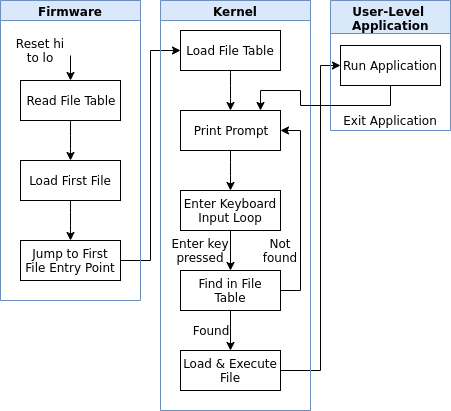
\includegraphics[width=10cm]{appflow.png}
\caption{Demonstration of application flow between firmware, kernel, and user level application.}
\label{appflow}
\end{figure}

Since the goal of this project is to emulate the functionality of a modern personal computer, the software is somewhat complicated. By design, it must be able to handle I/O and be able to load programs into memory and execute them. Because we wanted this system to be fully upgradable software-wise, the kernel, or operating system is not encoded into memory. It is only stored in the file system storage. Thus, our application consists of three main categories: firmware, kernel, and user level applications.

The firmware's only job is to load and execute the first program listed in the file system. This first program is the kernel, or operating system of the computer. This simple task does not need to be changed, and as such this is loaded into a read only portion of the memory and is executed on reset.

The kernel performs a more complicated task. After being executed, it enteres an input loop that is expecting the user to enter a string that corresponds to another file on the file system. This other file should refer to another program. When the user enters a command that exists on the file system,then it is loaded into memory and executed. The kernel has another job though, and that is to provide a library of subroutines that can be jumped to by the loaded program in order to manipulate data, or interact with the I/O.

Finally, the user level program, which can be anything. The open-ended nature of this design allows a programmer to create any simple program and run it on this hardware without necessarily knowing the ins and outs of the hardware. The idea is with a basic understanding of the memory map, any proficient assembly programmer should be able to use the kernel functions to accomplish the goals of a basic program. The flow of all of this software on the processor is specified in fig \ref{appflow}.



\subsection{Firmware}

Firmware package is preloaded into FPGA RAM. Firmware accesses file allocation table and finds the first and second entry. The length of the first entry is determined by the start address of the second address via software.

The firmware then loads the first file in the allocation table into memory starting at the first address. When the firmware has completed, the firmware jumps to the first memory address, handing control over to the kernel.

\subsection{Kernel}
The objective of the kernel is to provide a command-line interface for running programs that exist on the file system. The kernel provides all functions for interfacing with I/O that are called from within the kernel and from user programs executed on the processor.

\subsubsection{Subroutines}
There are various subroutines available to user programs that are described below.

\begin{figure}
\centering
\begin{tabular}{lllll}
\bf Family & \bf Function & \bf ARG1 & \bf ARG2 & \bf RET \\
& & \it r10 & \it r11 & \it r12 \\
String & .STR\_LEN & str\_addr &\\
& .STR\_EQ & str\_addr\_a & str\_addr\_b & are\_equal \\
& .STR\_CPY & str\_addr\_src & str\_addr\_dest \\
Keyboard & .CHECK\_KEY & key\_code &  & key\_data\\ 
& .KEY\_NUMPRESSED &  &  & key\_num \\ 
Flow & .DELAY & ticks &  & \\ 
& .PROMPT & &  & \\ 
Display & .PRINT\_STR & str\_addr\_src & str\_addr\_dest & \\
 & .PRINT\_WORD\_HEX & word\_addr\_src & str\_addr\_dest & \\
 & .SET\_PRINT\_COLOR & color\_code &  & \\ 
\end{tabular}
\caption{Table of public kernel subroutines.}
\label{fig:functions}
\end{figure}
\paragraph{String Functions}
\begin{itemize}
\item STR\_LEN(str\_addr):
	Accepts the starting address of a string, and counts characters until the null termination of the string, then returns the length of the string, excluding the null terminator, in the return register.
\item STR\_EQ(str\_addr\_a,str\_addr\_b):
	Accepts the addresses of two strings, and iterates through them until either they have two different characters at the same index, in which case a zero is returned, or until they have both terminated at the same point, in which case the strings are equal and a one is returned.
\item STR\_CPY(str\_addr\_src,str\_addr\_dest):
	Accepts two string addresses and copies a string from the source address to the destination address, stopping after the null terminator in the source string was reached.
\end{itemize}
\paragraph{Keyboard Functions}
\begin{itemize}
\item CHECK\_KEY(key\_code):
	Accepts a key code and checks to see if that key code is currently pressed. If the key is currently pressed, 1 will be returned, otherwise a zero will be returned. Non-blocking.
\item KEY\_NUMPRESSED():
	Will return the key code of the next pressed key. If more than one key is pressed, then usually the lexographically smaller (ASCII code closer to zero) key will be returned. Occasionally it will be possible for a higher lexographical key to be pressed, but this is unlikely. Blocking.
\end{itemize}
\paragraph{Flow Functions}
\begin{itemize}
\item DELAY(ticks):
	Accepts a number of ticks to delay by. A tick in this case is exactly 50000 clock cycles, or $\frac{50000}{50000000}=1$ms.
\item PROMPT():
	Returns execution flow to the kernel, effectively a way for a program to exit. The screen is not flushed except for the prompt line and above. Anything written below the prompt line will persist until another program is run.
\end{itemize}
\paragraph{Display Functions}
\begin{itemize}
\item PRINT\_STR(str\_addr\_src,str\_addr\_dest):
	Accepts two string addresses, and copies the string at the source to the location at the destination, with one exception. The color bits of every character copied to the screen will be set to the value saved when SET\_PRINT\_COLOR was called last.
\item PRINT\_WORD\_HEX(word,str\_addr\_hex):
	Accepts a word value stored in the word register, and the address to print the word to. This function writes starting at the destination address four characters, that is the hexadecimal representation of the word that was supplied to it.
\item SET\_PRINT\_COLOR(color\_code):
	Accepts a color code, stored in the lower 8 bits of the color\_code word. This is stored and all subsequent print functions called in the kernel will use this stored color. When reset, the color code is initialized to white letters on black background.
\end{itemize}
\subsection{User program}
The user program is similar to any program run on a modern machine. The programs are written to the SD card and are loaded into memory by the firmware. They define their own functionality, but it is expected that for I/O from the SD card, the program uses the kernel's defined SD card access functions. The keyboard input and VGA output are handled by shared memory, which the user program may access itself.

\subsection{Assembler considerations}
The assembler must handle jumps to kernel code by outputting label spec files that contain the relative memory addresses of all labels in the compiled code. These files can be linked against in subsequent compilations to ensure that user programs can be linked against kernel subroutines.
\subsubsection{Unified memory}
The processor is designed with a unified memory structure in order to load files into memory for execution. This allows us to easily include data for our program in assembly code. The assembler inserts data such as null terminated strings and 

\subsubsection{Assembler Use Flow \& Kernel Linking}
The assembler must support linking accross files via a linking file. The flow for compiling and creating user programs is as follows:
\begin{enumerate}
\item Assemble Kernel $\rightarrow$ kernel.hex, kernel.ln
\subitem kernel.ln is a text file that links a label with a memory address. This can be included in a user program assembly code, which allows the use of all labels from of kernel source assembly from within the user program code. It is similar to the a header file for the c standard library functions and memory addresses.
\item Assemble user program $\rightarrow$ prog.hex, prog.ln
\subitem The assembler checks if any undefined labels used in the user program code are defined in the linking file, if so the address from the link file is used.
\end{enumerate}
This system works without further hardware modification because the kernel is addressed by the firmware to start at address 0, so no offset is required for jumping to a kernel address. The link file also contains an end address, that is essentially the size in bytes of the compiled kernel code less one. This is used to calculate offsets for the user program's labels, since it exists above the kernel in memory.

This requires that all user programs are recompiled after a change to the kernel.
\subsection{Memory Map}
Because the processor is using unified memory, it is relatively simple to have multiple applications in memory on the device. In order for this to work well though, the memory map must be well defined so that applications do not step outside their boundaries, and so that the locations of common resources and kernel subroutines are known at compile time. This is necessary for user applications to be able to jump to kernel functions. Fig. \ref{fig:mmap} shows the memory boundaries for the different I/O memory sections as well as where the firmware, kernel, and user programs are located.
\begin{figure}
\centering
\begin{tikzpicture}

\node[draw, minimum width=40mm, minimum height=7mm, label=above:{Addr, Len}] (addr) {0x0000, kernel len};
\node[draw, minimum width=80mm, minimum height=7mm, right=-\pgflinewidth of addr, label=above:Description] (desc) {Kernel};

\node[draw, minimum width=40mm, minimum height=7mm,below=-\pgflinewidth of addr] (addr) {kernel len, prog len};
\node[draw, minimum width=80mm, minimum height=7mm, right=-\pgflinewidth of addr] (desc) {User program};

\node[draw, minimum width=40mm, minimum height=7mm,below=-\pgflinewidth of addr] (addr) {\ldots};
\node[draw, minimum width=80mm, minimum height=7mm, right=-\pgflinewidth of addr] (desc) {Empty};

\node[draw, minimum width=40mm, minimum height=7mm,below=-\pgflinewidth of addr] (addr) {0xC800, 512};
\node[draw, minimum width=80mm, minimum height=7mm, right=-\pgflinewidth of addr] (desc) {Kernel - user shared memory};

\node[draw, minimum width=40mm, minimum height=7mm,below=-\pgflinewidth of addr] (addr) {0xD000, 256};
\node[draw, minimum width=80mm, minimum height=7mm, right=-\pgflinewidth of addr] (desc) {Keyboard memory};

\node[draw, minimum width=40mm, minimum height=7mm,below=-\pgflinewidth of addr] (addr) {0xD800, 256};
\node[draw, minimum width=80mm, minimum height=7mm, right=-\pgflinewidth of addr] (desc) {Storage Memory};

\node[draw, minimum width=40mm, minimum height=7mm,below=-\pgflinewidth of addr] (addr) {0xE000, 4800};
\node[draw, minimum width=80mm, minimum height=7mm, right=-\pgflinewidth of addr] (desc) {VGA Glyph Memory};

\node[draw, minimum width=40mm, minimum height=7mm,below=-\pgflinewidth of addr] (addr) {0xFED3, 300};
\node[draw, minimum width=80mm, minimum height=7mm, right=-\pgflinewidth of addr] (desc) {Firmware - reset entry point!};
\end{tikzpicture}
\caption{Table showing memory layout of the processor design.}
\label{fig:mmap}
\end{figure}
\end{document}
